\section{Messung am Stockert}
\begin{frame}{Messung am Stockert}
  \begin{columns}[c, onlytextwidth]
    \begin{column}{0.4\textwidth}
      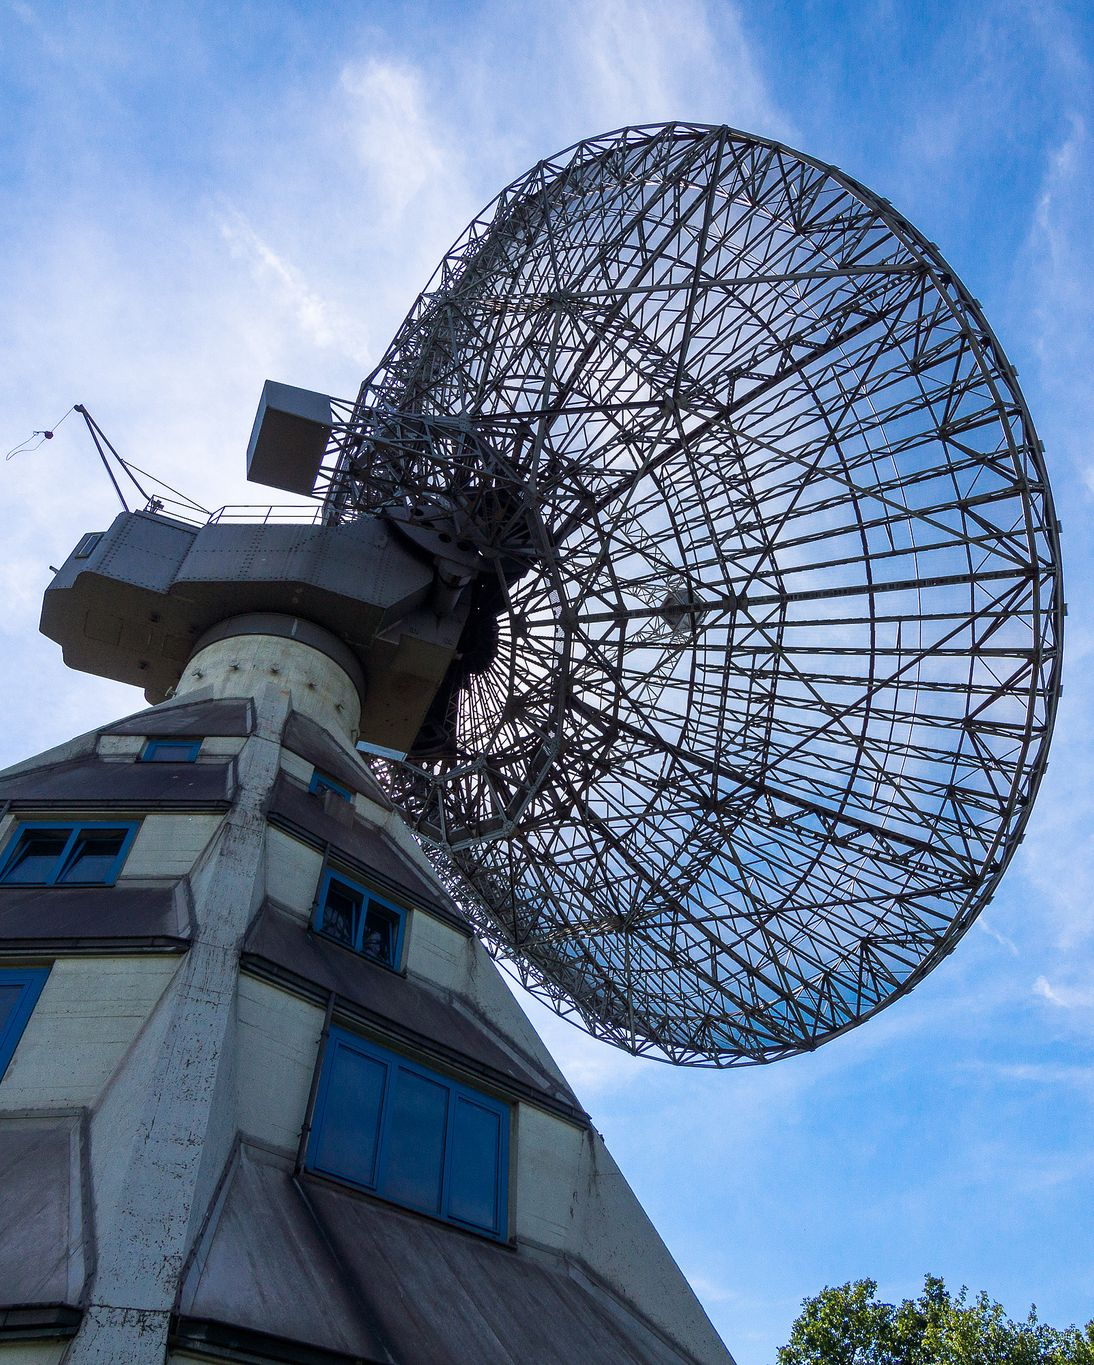
\includegraphics[width=\linewidth]{images/stockert_crop.jpg}
    \end{column}
    \begin{column}{0.55\textwidth}
      \begin{description}[Durchmesser]
        \item[Baujahr] 1956
        \item[Durchmesser] \SI{25}{\meter}
        \item[Auflösung]  \SI{0.5}{\degree} FWHM für $λ = \SI{21}{\centi\meter}$
        \item[Messung] Aufnahme von Spektren für verschiedene galaktische Längen
      \end{description}
    \end{column}
  \end{columns}
\end{frame}

\begin{frame}{Sichtbarkeit der Milchstraße}
  \begin{columns}[c, onlytextwidth]
    \begin{column}{0.65\textwidth}
      \begin{description}[15.6.2015]
        \item[1.6.2015] Arme in Zentrumsnähe ab ca. 20:30 Uhr \\
          Milchstraßen-Zentrum ca.\  22 – 4 Uhr
        \item[15.6.2015] Alle Zeiten ca.\ 30 Minuten früher
      \end{description}
    \end{column}
    \begin{column}{0.3\textwidth}
      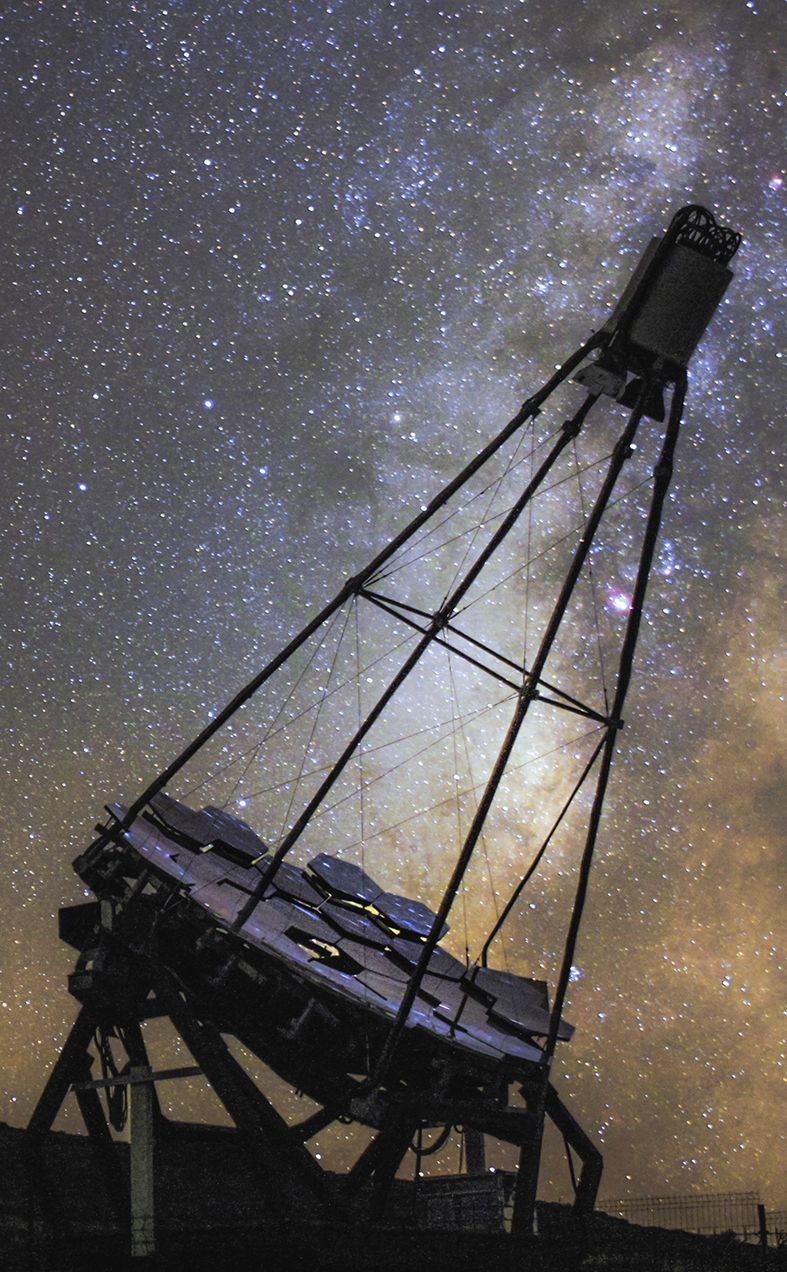
\includegraphics[width=\linewidth]{images/fact_crop.jpg}
    \end{column}
  \end{columns}
\end{frame}

\fullscreenimage[\color{darkred}1.6. 22:37 Uhr]{images/stellarium_20150601.jpg}
